\documentclass{article}

\usepackage[french]{babel}
\usepackage[T1]{fontenc}
\usepackage[a4paper,top=2cm,bottom=2cm,left=3cm,right=3cm,marginparwidth=1.75cm]{geometry}

% import packages
\usepackage{amsmath}
\usepackage{graphicx}
\usepackage{comment}
\usepackage[colorlinks=true, linkcolor=blue, urlcolor=purple]{hyperref}
\usepackage{float}
\usepackage{amsfonts}

\usepackage{tikz}
\usetikzlibrary{shapes.geometric, arrows, positioning}

\tikzstyle{layer} = [rectangle, draw, minimum width=3.5cm, minimum height=1cm, text centered]
\tikzstyle{inputnode} = [circle, draw=blue, fill=blue!20, minimum size=1.2cm, text centered]
\tikzstyle{outputnode} = [circle, draw=red, fill=red!20, minimum size=1.2cm, text centered]
\tikzstyle{arrow} = [thick, ->, >=stealth]

% title and author
\title{Rapport de Projet 8INF883}
\author{Cédric GAUTHERET}

% package for code listing
\usepackage{listings}
\usepackage{xcolor}

\definecolor{codegreen}{rgb}{0,0.6,0}
\definecolor{codegray}{rgb}{0.5,0.5,0.5}
\definecolor{codepurple}{rgb}{0.58,0,0.82}
\definecolor{backcolour}{rgb}{0.95,0.95,0.92}

\lstdefinestyle{mystyle}{
    backgroundcolor=\color{backcolour},   
    commentstyle=\color{codegreen},
    keywordstyle=\color{magenta},
    numberstyle=\tiny\color{codegray},
    stringstyle=\color{codepurple},
    basicstyle=\ttfamily\footnotesize,
    breakatwhitespace=false,         
    breaklines=true,
    frame=lines,
    captionpos=b,                    
    keepspaces=true,                 
    numbers=left,                    
    numbersep=5pt,                  
    showspaces=false,                
    showstringspaces=false,
    showtabs=false,                  
    tabsize=2
}

\lstset{style=mystyle}

\definecolor{light-gray}{gray}{0.95}

\newcommand{\code}[1]{\colorbox{light-gray}{\texttt{#1}}}

% dirtree package
\usepackage{dirtree}

\begin{document}

% page de garde
\begin{titlepage}
    \centering
    
    \text{ }
    \vspace{3cm}
    
    % Logos
    
\includegraphics[width=4cm]{logo_uqac.png}

    \vspace{2cm}

    \Huge\textbf{Rapport de Projet}\\[1.5cm]
    \Large\textbf{Projet Vision Artificielle et traitements des Images}\\[1cm]
    \Large \textbf{8INF883} \normalsize \\[1.5cm]

    \normalsize
    \textbf{Sujet :} Développement de modèles de génération de visages (CVAE / CGAN). \\[1.5cm]
    \textbf{Cédric GAUTHERET et Romain AMIGON}\\[0.5cm]

    \vfill

    \today

    \vspace{1cm}

\end{titlepage}


% --------------------
% table des matières
\newpage
\tableofcontents

\medskip
\medskip
\medskip
\medskip
\medskip

% --------------------

% --------------------
\newpage
\section{Introduction}

\subsection{Sujet}

L'objectif de notre projet est de faire de la génération d'image conditionnelle. On veut générer des visages comportant des attributs que l'on peut choisir selon une liste, par exemple on peut générer un visage de femme avec des lunettes et un chapeau.

\subsection{Motivations}

Ce projet peut s'inscrire dans une idée d'application, par exemple pour les opticiens coiffeurs ou pour des marchands de la mode.

En effet, on peut imaginer une application sur téléphone avec laquelle l'utilisateur peut prendre son visage et y ajouter la génération de lunette ou changer sa couleur de cheveux pour voir comment cela rend et se projeter avant de faire un achat.

\medskip

\noindent Ce projet sera l'occasion d'explorer les CGAN/DCGAN et CVAE.

\medskip

\noindent On utilisera pour ce projet le jeu de données \textbf{CelebA}.

\medskip
\medskip
\medskip

\textit{On va dans la suite de ce rapport, commenter certains éléments de code pour mieux comprendre nos implémentations, évidemment ce sera fait de manière non exhaustive pour ne pas le surcharger.}




\newpage
\section{Les données}

Le jeu de données (dataset) \textbf{CelebFaces Attributes (CelebA)} est un jeu de données à grande échelle d'attributs faciaux contenant plus de $200 000$ images de célébrités.

La grande force de cette base de données réside dans sa diversité : elle intègre d'importantes variations de poses, des arrière-plans complexes et désordonnés, ainsi qu'une grande variété de profils humains. Le tout est soutenu par un volume massif d'images et des annotations d'une grande richesse. \textit{(Ces données ont été initialement collectées par les chercheurs du MMLAB de l'Université chinoise de Hong Kong).}

\medskip

\noindent Les caractéristiques principales de ce jeu de données sont les suivantes :
\begin{itemize}
    \item Volume : $202 599$ images de visages.
    \item Identités : $10 177$ célébrités uniques.
    \item Annotations : $40$ attributs binaires par image (ex. : \textit{Souriant}, \textit{Lunettes}, \textit{Homme}, \textit{Jeune}).
    \item Repères (Landmarks) : 5 points de repère par image (yeux, nez, coins de la bouche).
\end{itemize}

\medskip

\textbf{CelebA} est une référence incontournable en vision par ordinateur pour l'entraînement des réseaux antagonistes génératifs (GAN). Sa grande diversité de poses, d'arrière-plans et de variations faciales le rend idéal pour générer des visages très réalistes.

\medskip

\noindent Le jeu de données se présente sous la forme suivante une fois téléchargé :

\begin{figure}[H]
    \centering
    \begin{minipage}{0.9\textwidth}
    \dirtree{%
        .1 CelebA/.
            .2 img\_align\_celeba/ \hfill \dots{} \textit{Répertoire principal des images}.
                .3 img\_align\_celeba/ \hfill \dots{} \textit{Sous-dossier contenant les fichiers .jpg}.
            .2 list\_attr\_celeba.csv \hfill \dots{} \textit{Attributs binaires (sourire, lunettes, etc.)}.
            .2 list\_bbox\_celeba.csv \hfill \dots{} \textit{Coordonnées des boîtes englobantes}.
            .2 list\_eval\_partition.csv \hfill \dots{} \textit{Répartition (train, valid, test)}.
            .2 list\_landmarks\_align\_celeba.csv \hfill \dots{} \textit{Points de repère faciaux (yeux, nez, bouche)}.
    }
    \end{minipage}
    \caption{Structure de l'arborescence du dataset CelebA}
    \label{fig:celeba_tree}
\end{figure}

\medskip

\texttt{img\_align\_celeba} : Le coeur du dataset. Il contient toutes les images de visages, qui ont déjà été recadrées et alignées (les yeux sont toujours à peu près au même niveau).

\medskip

\texttt{list\_eval\_partition.csv} : Ce fichier propose une répartition standardisée des images pour l'apprentissage :

\begin{itemize}
    \item Train : Images $1$ à $162 770$.
    \item Validation : Images $162 771$ à $182 637$.
    \item Test : Images $182 638$ à $202 599$.
\end{itemize}

\noindent \textit{Étant donné que l'on ne va pas faire de la classification mais de la génération d'image, on n'a pas besoin d'utiliser une telle répartition.}

\medskip

\texttt{list\_bbox\_celeba.csv} : Contient les informations des \textit{bounding boxes} permettant de localiser précisément le visage dans l'image d'origine. Les colonnes \code{x\_1} et \code{y\_1} indiquent les coordonnées du coin supérieur gauche de la boîte, tandis que \code{width} et \code{height} en définissent la largeur et la hauteur.

\medskip

\texttt{list\_landmarks\_align\_celeba.csv} : Fournit les coordonnées exactes (x, y) de 5 points clés du visage : l'oeil gauche, l'oeil droit, le nez, ainsi que les coins gauche et droit de la bouche.

\medskip

\texttt{list\_attr\_celeba.csv} : Le fichier des \textit{labels}. Il répertorie les 40 attributs de chaque image. La valeur \code{1} indique que l'attribut est présent (positif), tandis que la valeur \code{-1} indique son absence (négatif).

\medskip
\medskip

On a choisi ce dataset pour ses \textbf{40 attributs} qui permettent de conditionner un \textbf{CGAN}. Au lieu de générer des visages de manière purement aléatoire, nous pourrons utiliser ces étiquettes pour diriger le modèle et générer des visages "à la carte". Par exemple, on pourra demander spécifiquement au générateur de créer "un homme blond avec des lunettes" ou "une femme souriante".

Pour notre \textbf{CGAN} basé sur des réseaux convolutifs (\textbf{CNN}), nous devrons pré-traiter ces images. Nous allons les recadrer, les redimensionner à une taille standard et uniforme (ex. : 64x64), et normaliser la valeur de leurs pixels dans la plage [-1, 1] afin de correspondre à la fonction d'activation Tanh habituellement présente à la sortie du Générateur.

\subsection{Exploration}

On peut afficher les premières images pour avoir une idée de ce à quoi elles ressemblent dans le jeu de données.

\begin{figure}[H]
    \centering
    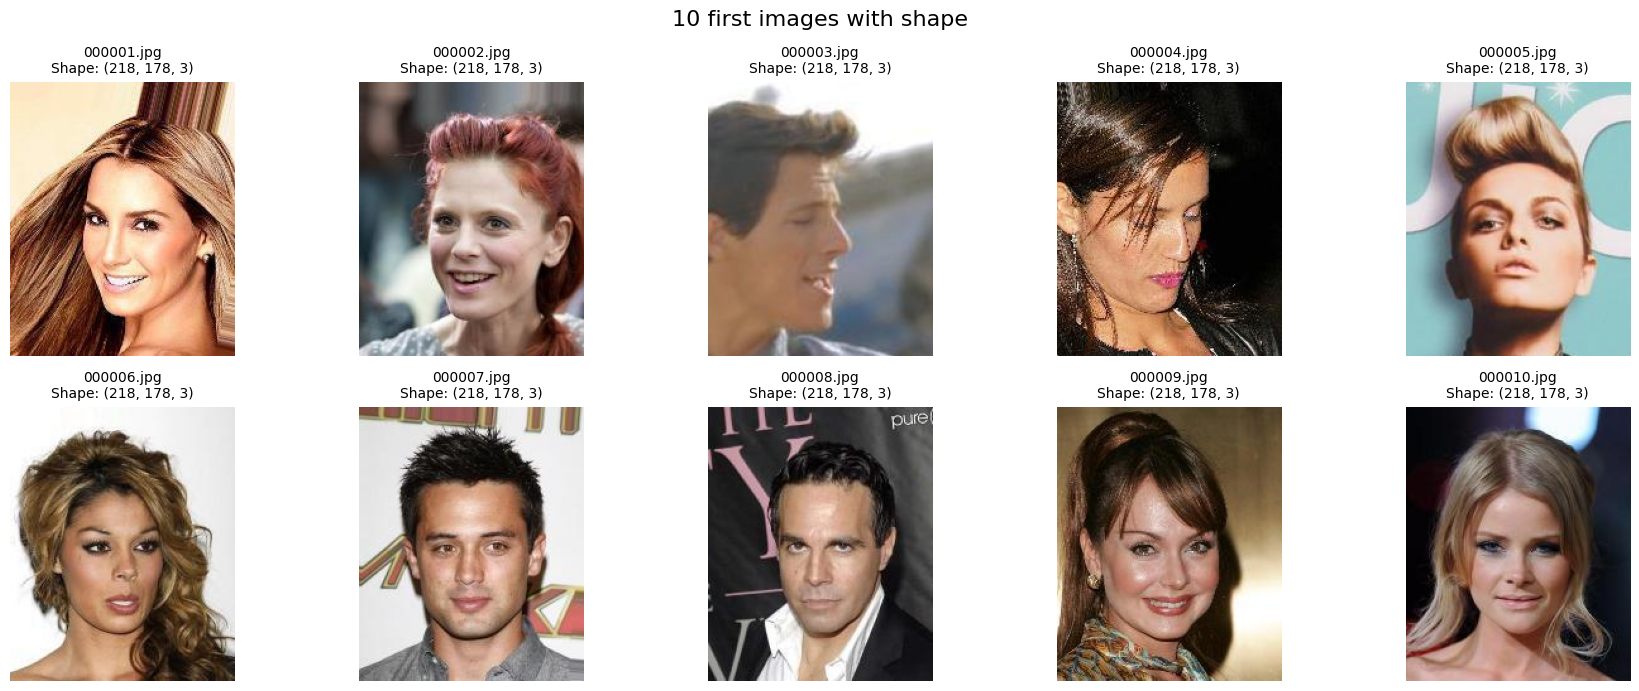
\includegraphics[width=1\textwidth]{data_head_10.png}
    \caption{Les 10 premières images et leur taille}
    \label{fig:data_head_10}
\end{figure}

On remarque que toutes les images ont la même taille : \code{(218, 178, 3)}.

\noindent Pour s'en assurer, on utilise le script suivant :

\medskip
\begin{lstlisting}[language=Python, caption={Vérification shape des images}]
unique_shapes = set()

for i, img_name in enumerate(img_names):
    img_path = os.path.join(img_dir, img_name)
    
    with Image.open(img_path) as img:
        channels = 3 if img.mode == 'RGB' else (1 if img.mode == 'L' else img.mode)
        shape = (img.size[1], img.size[0], channels)
        
        unique_shapes.add(shape)
        
print(f"Number of unique shapes found: {len(unique_shapes)}")

for shape in unique_shapes:
    print(f"- {shape}")
\end{lstlisting}

\noindent On vérifie donc que toutes les images ont la même taille : \code{218x178}.
Pour autant, on appliquera un redimensionnement dans notre pré-traitement pour diminuer la taille des images.

On peut aussi afficher la fréquence des attributs dans le jeu de données pour avoir une idée de la répartition (les images pouvant avoir plusieurs attributs).

\begin{figure}[H]
    \centering
    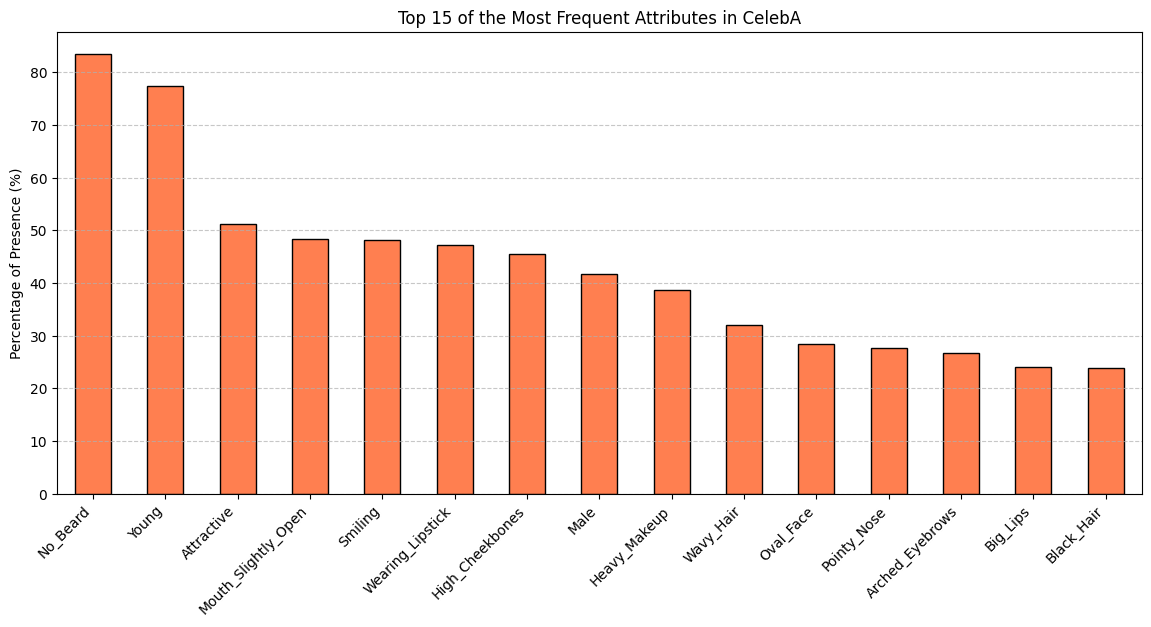
\includegraphics[width=1\textwidth]{attributes_chart.png}
    \caption{Fréquence des attributs}
    \label{fig:attributes_chart}
\end{figure}

\noindent On peut ainsi afficher les attributs qui sont les plus rares.

\medskip
\begin{lstlisting}
Most Rare Attributes :
Double_Chin    4.668829
Pale_Skin      4.294690
Gray_Hair      4.194986
Mustache       4.154512
Bald           2.244335
\end{lstlisting}

On remarque alors que la répartition est très inégale, certains attributs sont sur-représentés (proportionnellement) comme \code{No\_Beard} ou \code{Young} et d'autres sont sous-représentés et seront donc surement non utilisables comme \code{Bald} ou \code{Mustache}.

\noindent On retiendra par exemple : \code{Smiling}, \code{Male}, \code{No\_Beard}, \code{Wearing\_Lipstick}, \code{Eyeglasses}.

\medskip

\noindent Par ailleurs, on récupère la liste des 40 attributs

\medskip
\begin{lstlisting}
List of 40 unique attributes :

5_o_Clock_Shadow, Arched_Eyebrows, Attractive, Bags_Under_Eyes, Bald
Bangs, Big_Lips, Big_Nose, Black_Hair, Blond_Hair
Blurry, Brown_Hair, Bushy_Eyebrows, Chubby, Double_Chin
Eyeglasses, Goatee, Gray_Hair, Heavy_Makeup, High_Cheekbones
Male, Mouth_Slightly_Open, Mustache, Narrow_Eyes, No_Beard
Oval_Face, Pale_Skin, Pointy_Nose, Receding_Hairline, Rosy_Cheeks
Sideburns, Smiling, Straight_Hair, Wavy_Hair, Wearing_Earrings
Wearing_Hat, Wearing_Lipstick, Wearing_Necklace, Wearing_Necktie, Young
\end{lstlisting}

\subsection{Pré-traitements}

Avant d'appliquer la normalisation, la fonction \code{transforms.ToTensor()} convertit l'image brute (dont les pixels ont des valeurs entières comprises entre $0$ et $255$) en un tenseur PyTorch où les valeurs sont redimensionnées en nombres flottants compris entre $0.0$ et $1.0$.

\noindent Nous allons appliquer une normalisation avec une moyenne de $0.5$ et un écart-type de $0.5$.
\begin{itemize}
    \item[\textbf{Pour un pixel noir ($0.0$) :}] \code{(0.0 - 0.5) / 0.5 = -1.0}
    \item[\textbf{Pour un pixel blanc ($1.0$) :}] \code{(1.0 - 0.5) / 0.5 = 1.0}
\end{itemize}


\noindent Toutes les valeurs de nos images réelles sont désormais étalées de manière symétrique sur la plage [-1, 1].

Dans l'architecture classique d'un GAN, la toute dernière couche du \textbf{Générateur} utilise une fonction d'activation \textbf{Tanh}. 

\noindent La propriété mathématique de la fonction \textbf{Tanh} est de sortir exclusivement des valeurs comprises entre -1 et 1. 

\noindent Pour que le \textbf{Discriminateur} puisse faire son travail correctement et comparer de manière équitable les "fausses" images créées par le \textbf{Générateur} et les "vraies" images du dataset CelebA, on doit utiliser les mêmes échelles.

Les chercheurs ont en effet prouvé (notamment dans le papier de recherche fondateur du DCGAN \cite{dcgan15}) que l'utilisation de la plage [-1, 1] avec une activation Tanh aide le modèle à converger plus rapidement et de manière plus stable. Cela génère des images avec des contrastes plus forts et réduit le risque de disparition du gradient (\textit{vanishing gradient}) pendant l'entraînement par rapport à une plage [0, 1].

\medskip
\begin{lstlisting}[language=Python, caption={Chargement du dataset dans un \code{DataLoader} PyTorch}]
transform = transforms.Compose([
    transforms.Resize((IMAGE_SIZE, IMAGE_SIZE)),
    transforms.CenterCrop(IMAGE_SIZE),
    transforms.ToTensor(),
    transforms.Normalize(mean=(0.5, 0.5, 0.5), std=(0.5, 0.5, 0.5))
])

class CelebADataset(Dataset):
    def __init__(self, root_dir, attr_df, transform=None):
        self.root_dir = root_dir
        self.image_files = [f for f in os.listdir(root_dir) if f.endswith('.jpg')]
        self.attr_df = attr_df
        self.transform = transform

    def __len__(self):
        return len(self.image_files)

    def __getitem__(self, idx):
        img_name = self.image_files[idx]
        img_path = os.path.join(self.root_dir, img_name)
        
        image = Image.open(img_path).convert('RGB')
        if self.transform:
            image = self.transform(image)

        attributes = torch.tensor(self.attr_df.loc[img_name].values, dtype=torch.float32)
        
        return image, attributes
        
celeba_dataset = CelebADataset(root_dir=img_dir, attr_df=df_attr, transform=transform)

dataloader = DataLoader(
    celeba_dataset, 
    batch_size=BATCH_SIZE, 
    shuffle=True, 
    num_workers=0,
    pin_memory=True
)
\end{lstlisting}
\newpage
\section{Le modèle CGAN}

\noindent\rule{\linewidth}{0.4pt}

\noindent \textit{Le processus de création du GAN est documenté et disponible dans le notebook jupyter suivant :} \texttt{GAN/GAN.ipynb}

\noindent\rule{\linewidth}{0.4pt}

\subsection{Le modèle}

Un réseau antagoniste génératif classique repose sur une compétition féroce entre deux modèles de neurones.

\begin{figure}[H]
    \centering
    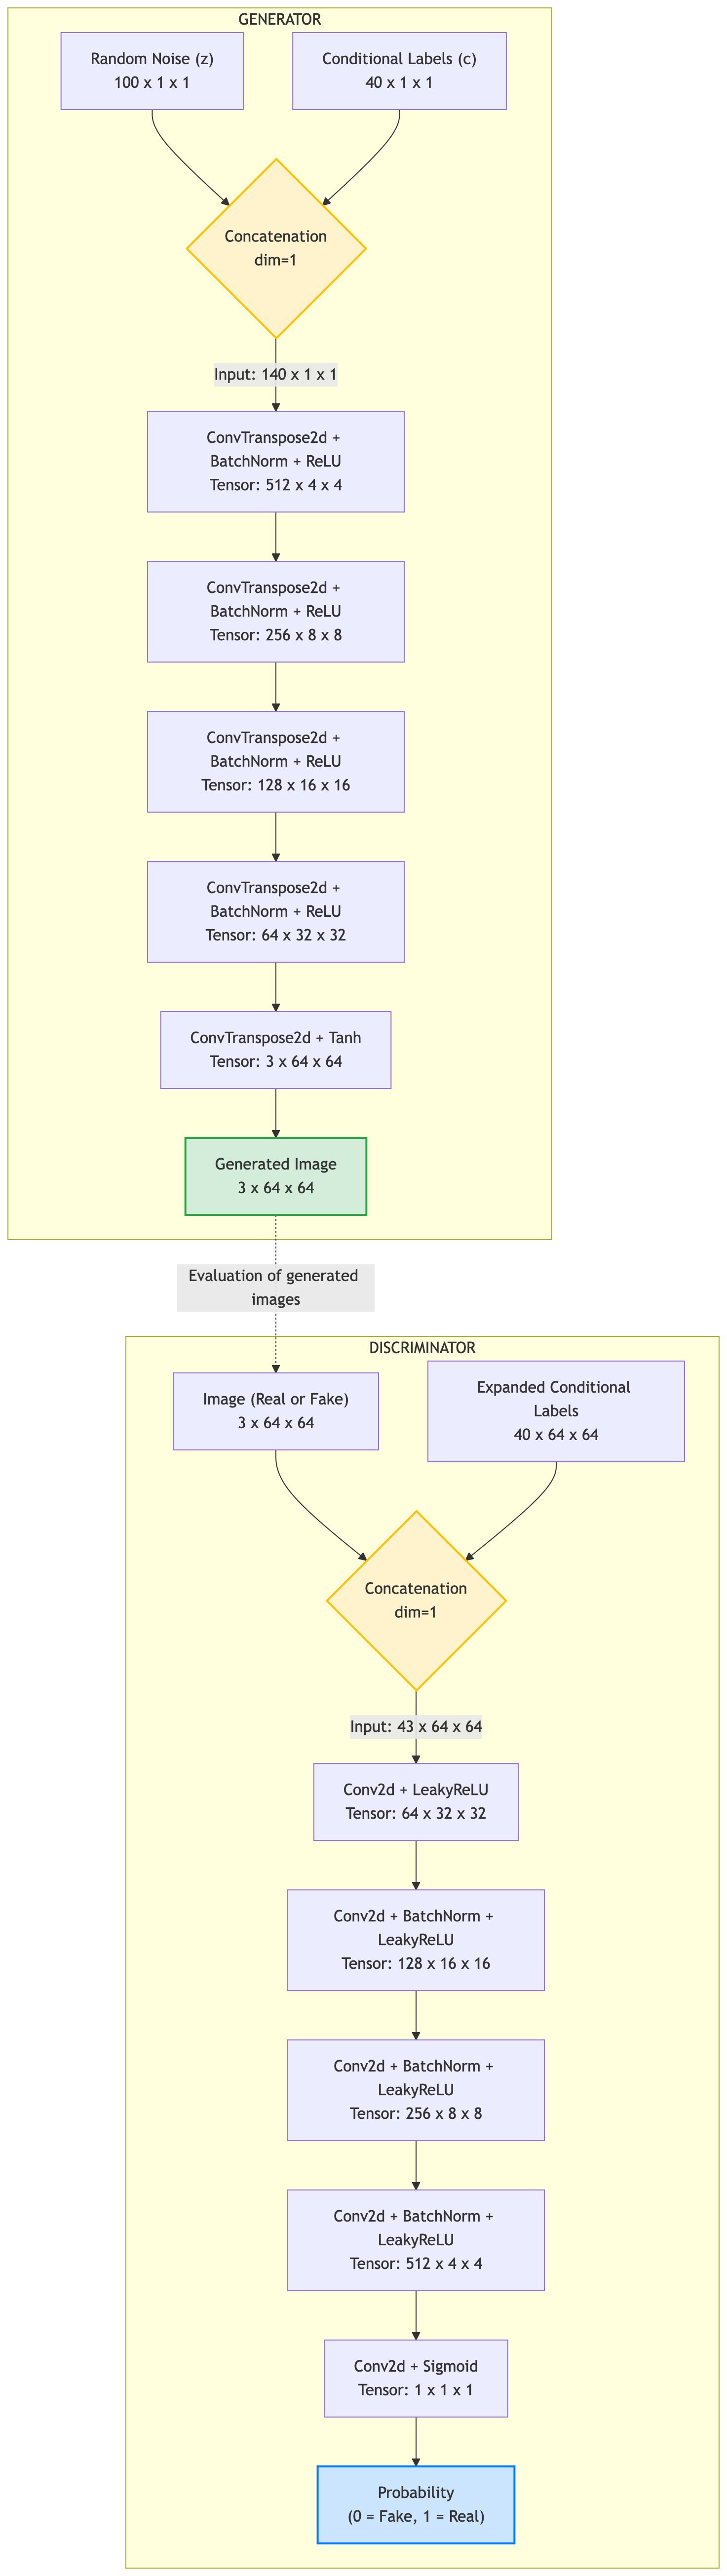
\includegraphics[height=1.3\textwidth]{GAN_model.png}
    \caption{Architecture du CGAN}
    \label{fig:GAN_model}
\end{figure}

\newpage
Le premier est le \textbf{Générateur}, dont le but est de transformer un vecteur de bruit aléatoire abstrait, noté $z$, en une donnée réaliste, comme une image. 
Le second est le \textbf{Discriminateur}, qui agit comme un détective cherchant à séparer les véritables images provenant de la base de données de celles fabriquées par le Générateur. 

\medskip

Dans un Conditional GAN, ou \textbf{CGAN}, cette dynamique est enrichie par l'ajout d'une information supplémentaire, notée $c$, qui représente une condition. Au lieu de générer des visages au hasard, le modèle apprend à lier des caractéristiques visuelles spécifiques à cette variable $c$. Mathématiquement, cette compétition se modélise par une fonction objectif \textbf{minimax} où le \textbf{Générateur} tente de minimiser la fonction que le Discriminateur cherche à maximiser. 

L'équation fondamentale du CGAN s'écrit donc 

$$\min_G \max_D V(D, G) = \mathbb{E}_{x \sim p_{data}(x)}[\log D(x|c)] + \mathbb{E}_{z \sim p_z(z)}[\log(1 - D(G(z|c)|c))]$$

Pour arbitrer ce jeu, nous utilisons la Binary Cross Entropy Loss, ou \textbf{BCELoss}. 

Étant donné que le rôle final du \textbf{Discriminateur} est de déterminer si une image est vraie ou fausse, le problème se résume à une classification binaire classique. La fonction Sigmoïde placée à la toute fin du réseau du \textbf{Discriminateur} comprime la sortie pour fournir une probabilité continue comprise entre $0$ et $1$. La \textbf{BCELoss} va alors mesurer la distance mathématique entre cette probabilité prédite et la véritable étiquette de l'image. 

Soit, 
$$\mathcal{L}_{BCE} = - \frac{1}{N} \sum_{i=1}^{N} \left[ y_i \log(\hat{y}_i) + (1 - y_i) \log(1 - \hat{y}_i) \right]$$ 

où $y_i$ représente l'étiquette réelle, valant $1$ pour une vraie image et $0$ pour une fausse, tandis que $\hat{y}_i$ représente la prédiction du modèle. 

Lors de l'entraînement, le \textbf{Discriminateur} cherche à minimiser cette erreur par rapport à la réalité, tandis que le Générateur calcule sa propre perte en passant ses fausses images au \textbf{Discriminateur} mais en cherchant à minimiser l'erreur par rapport à l'étiquette cible $1$, forçant ainsi le modèle à s'améliorer pour tromper son adversaire.

\medskip

Dans notre implémentation, le Générateur est conçu selon les principes de l'architecture \textbf{DCGAN} (\cite{dcgan15}), basée sur des convolutions profondes. Tout commence par la fusion de nos entrées. Nous prenons notre vecteur de bruit de dimension $100$ et le concaténons directement avec notre vecteur de conditions de dimension $40$. Le réseau démarre donc avec un volume d'entrée de dimension $140 \times 1 \times 1$. Pour transformer ce minuscule bloc d'informations en une image complète, nous utilisons des couches de convolutions transposées. Ces couches agissent à l'inverse des convolutions classiques en effectuant un suréchantillonnage spatial. À chaque étape, la résolution de notre image en devenir est doublée, passant de $4 \times 4$, puis $8 \times 8$, jusqu'à atteindre notre objectif de $64 \times 64$ pixels. 

Après presque chaque convolution, nous appliquons une normalisation par lot, ou \textit{BatchNorm}, qui standardise les activations internes et empêche le modèle de diverger de manière chaotique lors des premières phases d'apprentissage. La non-linéarité est assurée par la fonction ReLU qui accélère la convergence. Enfin, la toute dernière couche utilise une activation Tanh pour forcer la sortie mathématique à se situer strictement dans l'intervalle $[-1, 1]$, correspondant exactement à l'échelle de normalisation que nous avons appliquée à nos images réelles lors du prétraitement.

Le \textbf{Discriminateur} effectue exactement le cheminement inverse. Puisqu'il est impossible de concaténer simplement un vecteur unidimensionnel de taille $40$ avec une image bidimensionnelle de taille $64 \times 64$, l'architecture commence par répéter le vecteur conditionnel sur toute la surface de l'image. Cela crée $40$ nouveaux canaux d'information, empilés virtuellement derrière les $3$ canaux de couleur RGB de l'image. La première couche de convolution reçoit donc une pile de données de $43$ canaux. Le réseau utilise ensuite une série de convolutions standards avec un pas, ou \textit{stride}, de $2$. 

Ce choix architectural volontaire remplace les traditionnelles opérations de \textit{MaxPooling}, laissant au réseau la liberté d'apprendre par lui-même la meilleure méthode pour réduire la résolution spatiale à chaque étape. Une caractéristique vitale de ce \textbf{Discriminateur} est l'utilisation exclusive de l'activation \textit{LeakyReLU} avec une pente négative de $0.2$. Contrairement au ReLU standard qui met purement et simplement à zéro toutes les valeurs négatives, le LeakyReLU laisse passer un infime flux d'information. Cette astuce empêche le \textbf{Discriminateur} de bloquer complètement la circulation des gradients, garantissant que le Générateur reçoive toujours un retour d'information mathématique pour corriger ses erreurs, même lorsque ses fausses images sont facilement démasquées au début de l'entraînement.

\subsubsection*{Le Générateur}

Pour que le modèle prenne en compte les 40 attributs faciaux ($c$), le Générateur intègre l'information conditionnelle dès l'entrée du réseau : le vecteur de bruit aléatoire $z \in \mathbb{R}^{100}$ est concaténé avec le vecteur d'attributs $c \in \mathbb{R}^{40}$, formant ainsi un vecteur global de taille $140$. L'objectif est de transformer ce vecteur latent en une image complexe de $64 \times 64$ pixels. Pour ce faire, le réseau utilise des couches de convolutions transposées (\code{nn.ConvTranspose2d()}) qui augmentent la résolution spatiale par étapes successives (de $4 \times 4$ jusqu'à $64 \times 64$). Chaque couche est suivie d'une normalisation par lot (\code{nn.BatchNorm2d()}) afin de standardiser les activations intermédiaires, stabilisant ainsi l'apprentissage et facilitant la circulation des gradients. Alors que les couches cachées utilisent l'activation \code{nn.ReLU()} pour introduire des non-linéarités sans saturer, la couche de sortie emploie la fonction tangente hyperbolique (\code{nn.Tanh()}). Ce choix contraint les pixels générés dans la plage $[-1, 1]$, assurant une cohérence parfaite avec le prétraitement appliqué aux images réelles.

\medskip

Le choix de la profondeur des réseaux et de l'évolution des dimensions des \textit{feature maps} repose sur un équilibre entre complexité et stabilité de convergence. Pour une résolution cible de $64 \times 64$ pixels, une architecture à cinq blocs de convolution est standard : elle permet une réduction (ou augmentation) progressive par puissances de deux ($2^2 \to 2^6$). Dans le Générateur, le choix de débuter avec \code{FEATURES\_GEN} $\times 8$ (512 canaux) pour finir à 3 canaux permet de condenser l'information sémantique complexe des 140 variables d'entrée dans un grand nombre de filtres initiaux, avant de les projeter vers une structure spatiale plus large mais moins profonde. Cette décompression progressive est essentielle pour que le réseau puisse d'abord générer des formes globales cohérentes avant de s'affiner sur les détails texturaux.


\medskip
\begin{lstlisting}[language=Python, caption={Architecture du \textbf{Générateur}}]
class Generator(nn.Module):
    def __init__(self, z_dim, c_dim, features_g):
        super(Generator, self).__init__()
        # Input to the first layer is noise (z_dim) + condition (c_dim)
        in_channels = z_dim + c_dim
        
        self.gen = nn.Sequential(
            # Input: (in_channels) x 1 x 1
            nn.ConvTranspose2d(in_channels, features_g * 8, kernel_size=4, stride=1, padding=0, bias=False),
            nn.BatchNorm2d(features_g * 8),
            nn.ReLU(True),
            
            # State: (features_g*8) x 4 x 4
            nn.ConvTranspose2d(features_g * 8, features_g * 4, kernel_size=4, stride=2, padding=1, bias=False),
            nn.BatchNorm2d(features_g * 4),
            nn.ReLU(True),
            
            # State: (features_g*4) x 8 x 8
            nn.ConvTranspose2d(features_g * 4, features_g * 2, kernel_size=4, stride=2, padding=1, bias=False),
            nn.BatchNorm2d(features_g * 2),
            nn.ReLU(True),
            
            # State: (features_g*2) x 16 x 16
            nn.ConvTranspose2d(features_g * 2, features_g, kernel_size=4, stride=2, padding=1, bias=False),
            nn.BatchNorm2d(features_g),
            nn.ReLU(True),
            
            # State: (features_g) x 32 x 32
            nn.ConvTranspose2d(features_g, CHANNELS, kernel_size=4, stride=2, padding=1, bias=False),
            # Output uses Tanh to map values to [-1, 1]
            nn.Tanh()
            # Final output: 3 x 64 x 64
        )

    def forward(self, x, labels):
        # Reshape labels to append them to the latent noise vector
        labels = labels.unsqueeze(2).unsqueeze(3) # Shape: (batch, C_DIM, 1, 1)
        # Concatenate noise and labels along the channel dimension
        x = torch.cat([x, labels], dim=1)
        return self.gen(x)
\end{lstlisting}

\subsubsection*{Le Discriminateur}

Le Discriminateur agit comme un classifieur binaire dont l'entrée est hybride : il doit analyser à la fois la structure de l'image et sa correspondance avec les attributs. Le vecteur $c$ est "étiré" spatialement pour créer 40 canaux (calques) à la taille de l'image ($64 \times 64$). Le réseau traite donc un bloc de données composé de $3$ canaux de couleurs (RGB) et de 40 canaux de conditions, soit un total de $43$ canaux en entrée. Le sous-échantillonnage est effectué via des convolutions avec un pas de deux (\code{stride=2}), permettant au modèle d'apprendre sa propre réduction de dimension plutôt que d'utiliser un \textit{MaxPooling} figé. Conformément aux recommandations DCGAN (\cite{dcgan15}), la première couche ne comporte pas de \code{nn.BatchNorm()} pour préserver la distribution brute des données. L'activation \code{nn.LeakyReLU()} avec une pente de $0.2$ est systématiquement privilégiée pour éviter le problème des "neurones morts", tandis qu'une \code{nn.Sigmoid()} finale fournit la probabilité d'authenticité. L'ensemble est entraîné avec l'optimiseur Adam ($lr=0.0002$, $\beta_1=0.5$), des paramètres hyper-spécifiques cruciaux pour prévenir les instabilités et les oscillations communes lors de l'entraînement des GANs.

\medskip

Côté Discriminateur, la structure symétrique commençant à \code{FEATURES\_DISC} (64 canaux) permet de capturer d'abord des motifs locaux simples (bords, couleurs), puis d'augmenter la profondeur à chaque réduction spatiale pour extraire des caractéristiques de plus en plus abstraites et globales. L'utilisation d'une base de 64 filtres (\code{FEATURES\_GEN/DISC}) offre un compromis optimal : elle fournit suffisamment de paramètres pour modéliser la diversité du dataset CelebA (variété de visages, poses et éclairages) sans pour autant atteindre une complexité de calcul qui rendrait l'entraînement prohibitif ou sujet à un surapprentissage rapide. Ce dimensionnement garantit que le Discriminateur est assez puissant pour guider le Générateur sans devenir "trop fort" trop rapidement, évitant ainsi la disparition du gradient indispensable à la mise à jour des poids du Générateur.

\medskip
\begin{lstlisting}[language=Python, caption={Architecture du \textbf{Discriminateur}}]
class Discriminator(nn.Module):
    def __init__(self, c_dim, features_d):
        super(Discriminator, self).__init__()
        # Input channels = image channels (3) + condition channels (40)
        in_channels = CHANNELS + c_dim
        
        self.disc = nn.Sequential(
            # Input: (in_channels) x 64 x 64
            nn.Conv2d(in_channels, features_d, kernel_size=4, stride=2, padding=1, bias=False),
            nn.LeakyReLU(0.2, inplace=True),
            
            # State: (features_d) x 32 x 32
            nn.Conv2d(features_d, features_d * 2, kernel_size=4, stride=2, padding=1, bias=False),
            nn.BatchNorm2d(features_d * 2),
            nn.LeakyReLU(0.2, inplace=True),
            
            # State: (features_d*2) x 16 x 16
            nn.Conv2d(features_d * 2, features_d * 4, kernel_size=4, stride=2, padding=1, bias=False),
            nn.BatchNorm2d(features_d * 4),
            nn.LeakyReLU(0.2, inplace=True),
            
            # State: (features_d*4) x 8 x 8
            nn.Conv2d(features_d * 4, features_d * 8, kernel_size=4, stride=2, padding=1, bias=False),
            nn.BatchNorm2d(features_d * 8),
            nn.LeakyReLU(0.2, inplace=True),
            
            # State: (features_d*8) x 4 x 4
            nn.Conv2d(features_d * 8, 1, kernel_size=4, stride=1, padding=0, bias=False),
            nn.Sigmoid() # Output a probability [0, 1]
        )

    def forward(self, x, labels):
        # Expand labels to match the image spatial dimensions (64x64)
        labels = labels.unsqueeze(2).unsqueeze(3)
        labels = labels.repeat(1, 1, x.size(2), x.size(3)) # Shape: (batch, C_DIM, 64, 64)
        # Concatenate image and expanded labels
        x = torch.cat([x, labels], dim=1)
        return self.disc(x)
\end{lstlisting}


\subsection{Entraînements et résultats}

\noindent On définit la boucle d'entraînement suivante :

\medskip
\begin{lstlisting}[language=Python, caption={Entraînement du CGAN}]
def train_cgan(gen, disc, dataloader, device, num_epochs=5, z_dim=100):
    """
    Trains the Conditional GAN and returns the loss history.
    """
    # optimizers
    opt_gen = optim.Adam(gen.parameters(), lr=0.0002, betas=(0.5, 0.999))
    opt_disc = optim.Adam(disc.parameters(), lr=0.0002, betas=(0.5, 0.999))

    # loss function
    criterion = nn.BCELoss()

    # lists to keep track of progress
    G_losses = []
    D_losses = []

    for epoch in range(num_epochs):
        for batch_idx, (real_images, labels) in enumerate(dataloader):
            
            real_images = real_images.to(device)
            labels = labels.to(device)
            batch_size = real_images.shape[0]

            # Targets for BCE Loss (1 for real, 0 for fake)
            # we use a slight label smoothing (0.9 instead of 1.0) for real images to stabilize training
            real_targets = torch.full((batch_size, 1, 1, 1), 0.9, device=device)
            fake_targets = torch.zeros((batch_size, 1, 1, 1), device=device)

            # =========================================================
            # Train Discriminator: Maximize log(D(x)) + log(1 - D(G(z)))
            # =========================================================
            disc.zero_grad()
            
            # loss on real images
            output_real = disc(real_images, labels)
            loss_disc_real = criterion(output_real, real_targets)
            
            # loss on fake images
            # generate random noise
            noise = torch.randn(batch_size, z_dim, 1, 1, device=device)
            # generate fake images conditioned on the real labels
            fake_images = gen(noise, labels)
            
            output_fake = disc(fake_images.detach(), labels) # detach() prevents gradients from flowing into Generator
            loss_disc_fake = criterion(output_fake, fake_targets)
            
            # total Discriminator loss and backprop
            loss_disc = (loss_disc_real + loss_disc_fake) / 2
            loss_disc.backward()
            opt_disc.step()

            # =========================================================
            # Train Generator: Maximize log(D(G(z)))
            # =========================================================
            gen.zero_grad()
            
            # we want the discriminator to believe our fake images are real (target = 1)
            output_fake_for_gen = disc(fake_images, labels)
            
            loss_gen = criterion(output_fake_for_gen, torch.ones_like(output_fake_for_gen))
            loss_gen.backward()
            opt_gen.step()

            # save losses for plotting later
            G_losses.append(loss_gen.item())
            D_losses.append(loss_disc.item())

    # return the recorded losses
    return G_losses, D_losses
\end{lstlisting}

\subsubsection{Entraînement 5 époques (premiers tests)}

On va faire un premier entraînement sur 5 époques pour tester notre architecture et valider le modèle.

\medskip
\begin{lstlisting}[language=Python, caption={Entraînement du CGAN sur 5 époques}]
gen_5 = Generator(Z_DIM, C_DIM, FEATURES_GEN).to(device)
disc_5 = Discriminator(C_DIM, FEATURES_DISC).to(device)

NUM_EPOCHS = 5

G_losses_5, D_losses_5 = train_cgan(gen_5, disc_5, dataloader, device, num_epochs=NUM_EPOCHS, z_dim=Z_DIM)
\end{lstlisting}

\begin{figure}[H]
    \centering
    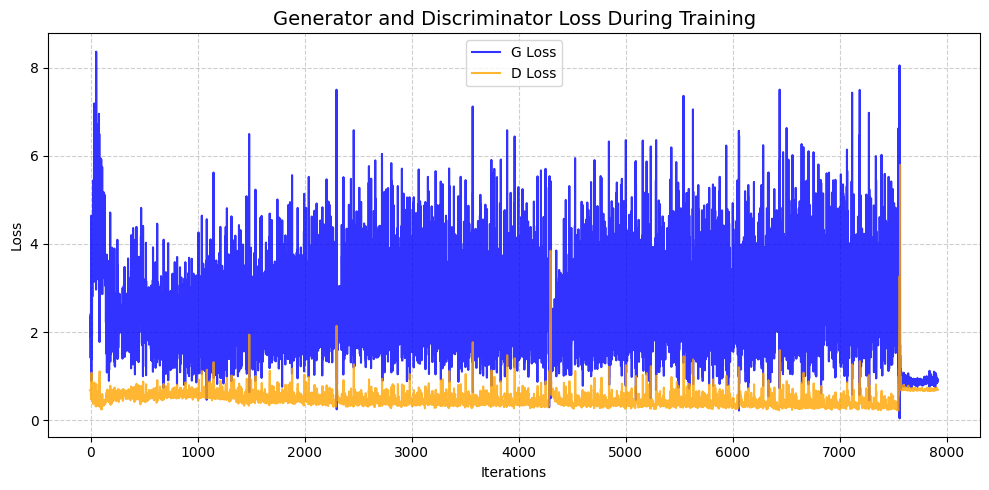
\includegraphics[width=1\textwidth]{loss_CGAN_5.png}
    \caption{Courbes de Loss du CGAN sur 5 époques}
    \label{fig:loss_CGAN_5}
\end{figure}

On remarque que la loss commence à se stabiliser vers la fin de l'entraînement ce qui est un bon signe.

\begin{figure}[H]
    \centering
    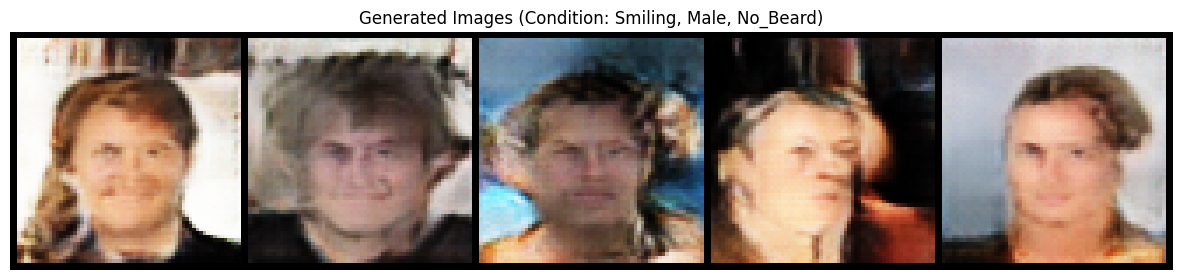
\includegraphics[width=1\textwidth]{test1_CGAN_5.png}
    \caption{Exemple avec attributs : \texttt{Smiling}, \texttt{Male} et \texttt{No\_Beard}}
    \label{fig:test1_CGAN_5}
\end{figure}

\begin{figure}[H]
    \centering
    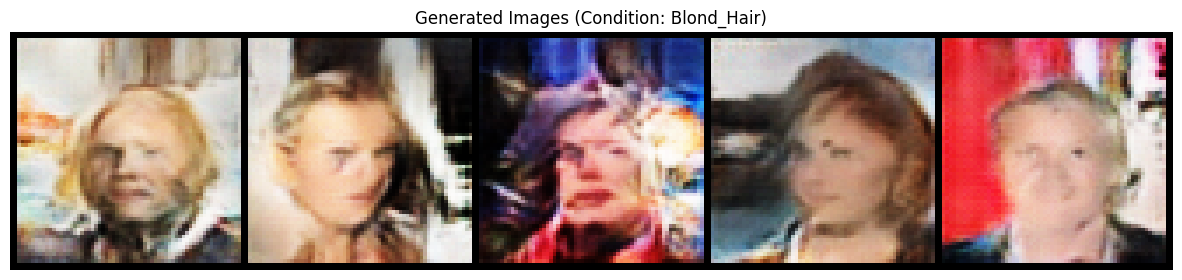
\includegraphics[width=1\textwidth]{test2_CGAN_5.png}
    \caption{Exemple avec attribut \texttt{Blond\_Hair}}
    \label{fig:test2_CGAN_5}
\end{figure}

Les résultats que l'on obtient sont prometteur, le modèle généralise suffisamment pour générer à chaque fois des visages différents et dans le cas d'un seul attribut : \texttt{Blond\_Hair}, on devine en effet l'attribut sur les images.

Pour tester la diversité du modèle et l'évaluer, on peut utiliser \textbf{LPIPS}.

\subsubsection{LPIPS}

Pour comparer les images de manière plus formelle, on peut utiliser \textbf{LPIPS}.

Au lieu de comparer les pixels bruts, LPIPS (Learned Perceptual Image Patch Similarity) utilise un réseau de neurones pré-entraîné (généralement VGG16 ou AlexNet, entraîné sur des millions d'images réelles avec ImageNet) comme "oeil humain" pour comparer les images.

\medskip

\noindent LPIPS suit le processus suivant :

\begin{itemize}
    \item \textbf{Extraction des caractéristiques :} Les deux images à comparer passent à travers le réseau VGG.
    \item \textbf{Récupération des activations :} LPIPS ne regarde pas la classification finale du réseau, mais s'arrête aux couches intermédiaires (les couches de convolution). Il extrait les \textit{feature maps}, qui représentent les textures, les formes et les couleurs perçues par le réseau (espace latent).
    \item \textbf{Calcul de la distance :} La métrique calcule la distance euclidienne entre ces cartes de caractéristiques pour chaque couche $l$, souvent pondérée par un vecteur $w$
\end{itemize}

\noindent Le calcul de la distance se fait selon la formule suivante :

$$d(x, x_0) = \sum_{l} \frac{1}{H_l W_l} \sum_{h, w} || w_l \odot (\hat{y}_{hw}^l - \hat{y}_{0hw}^l) ||_2^2$$

\noindent où $\hat{y}$ représente les activations du réseau pour l'image $x$, et $\hat{y}_0$ les activations pour l'image $x_0$.

\medskip
\begin{lstlisting}[language=Python, caption={Algo de score LPIPS}]
def compute_generation_diversity(generator, base_condition, device, num_pairs=10):
    generator.eval()
    lpips_metric = LearnedPerceptualImagePatchSimilarity(net_type='vgg').to(device)
    
    lpips_scores = []
    
    with torch.no_grad():
        for _ in range(num_pairs):
            # generate two different images using the exact same condition
            noise1 = torch.randn(1, Z_DIM, 1, 1, device=device)
            noise2 = torch.randn(1, Z_DIM, 1, 1, device=device)
            
            # we need batch size 1 for the condition here
            cond = base_condition[0].unsqueeze(0)
            
            img1 = generator(noise1, cond)
            img2 = generator(noise2, cond)
            
            # LPIPS expects images in range [-1, 1], which matches our generator output
            score = lpips_metric(img1, img2)
            lpips_scores.append(score.item())
            
    avg_lpips = sum(lpips_scores) / len(lpips_scores)
    print(f"Average LPIPS Diversity Score (Higher is better): {avg_lpips:.4f}")
\end{lstlisting}

Contrairement à la précision (où plus haut = meilleur), LPIPS est une mesure de distance :
\begin{itemize}
    \item[\textbf{LPIPS proche de 0 :}] Les deux images sont perceptuellement identiques.
    \item[\textbf{LPIPS élevé (ex: > 0.5) :}] Les deux images sont structurellement et visuellement très différentes.
\end{itemize}

\medskip

Dans le cas d'un CGAN, nous n'avons pas d'image "cible" exacte pour calculer une erreur. Si on demande au modèle de générer "un homme à lunettes", il n'y a pas une seule bonne réponse, il en existe des millions.

\medskip

\noindent Nous allons donc faire un test de diversité : nous donnons au Générateur la "même condition" (ex: "Femme, Souriante, Jeune") mais avec deux vecteurs de bruit différents ($z_1$ et $z_2$). Le modèle doit générer deux femmes différentes qui respectent ces critères. Nous calculons le score LPIPS entre ces deux images générées.

Si le LPIPS est très bas, cela signifie que le GAN a triché. Il a mémorisé un seul visage de "Femme souriante" et le recrache en boucle peu importe le bruit $z$.

\medskip

Si le LPIPS est suffisamment élevé, cela prouve que le Générateur a bien appris la distribution globale et est capable d'inventer des visages variés et uniques pour une même condition.

Dans notre contexte d'évaluation de la diversité interne d'un GAN, un score LPIPS plus élevé indique une bonne performance.

\medskip

\noindent\rule{\linewidth}{0.4pt}

\noindent Pour l'entraînement sur 5 époques, on obtient un score de $0.5899$.

\noindent\rule{\linewidth}{0.4pt}


\subsubsection{Entraînement 30 époques}

Dans l'article classique du DCGAN (\cite{dcgan15}), il est conseillé de faire un entraînement de 20 à 50 époques, je vais donc tester un entraînement sur 30 époques.

\medskip
\begin{lstlisting}[language=Python, caption={Entraînement du CGAN sur 30 époques}]
gen_30 = Generator(Z_DIM, C_DIM, FEATURES_GEN).to(device)
disc_30 = Discriminator(C_DIM, FEATURES_DISC).to(device)

NUM_EPOCHS = 30

G_losses_30, D_losses_30 = train_cgan(gen_30, disc_30, dataloader, device, num_epochs=NUM_EPOCHS, z_dim=Z_DIM)
\end{lstlisting}

\begin{figure}[H]
    \centering
    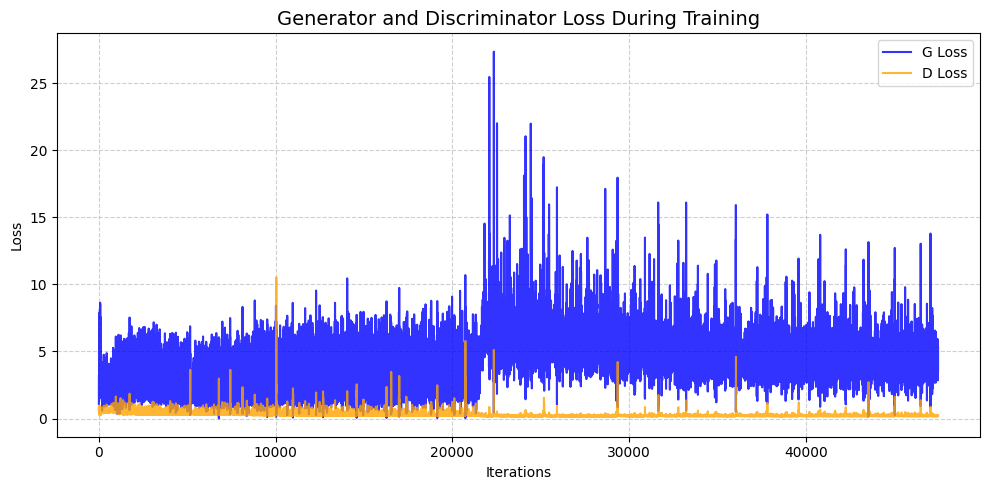
\includegraphics[width=1\textwidth]{loss_CGAN_30.png}
    \caption{Courbes de Loss du CGAN sur 30 époques}
    \label{fig:loss_CGAN_30}
\end{figure}

On remarque que passé un certain nombre d'époques, le modèle commence à diverger, on a un saut dans la loss. C'est le signe d'un sur-apprentissage ou d'un \textit{Gradient Exploding}.

\begin{figure}[H]
    \centering
    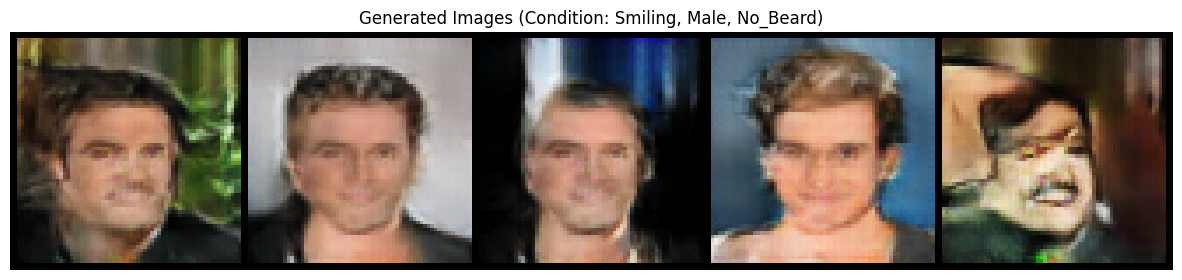
\includegraphics[width=1\textwidth]{test1_CGAN_30.png}
    \caption{Exemple avec attributs : \texttt{Smiling}, \texttt{Male} et \texttt{No\_Beard}}
    \label{fig:test1_CGAN_30}
\end{figure}

\begin{figure}[H]
    \centering
    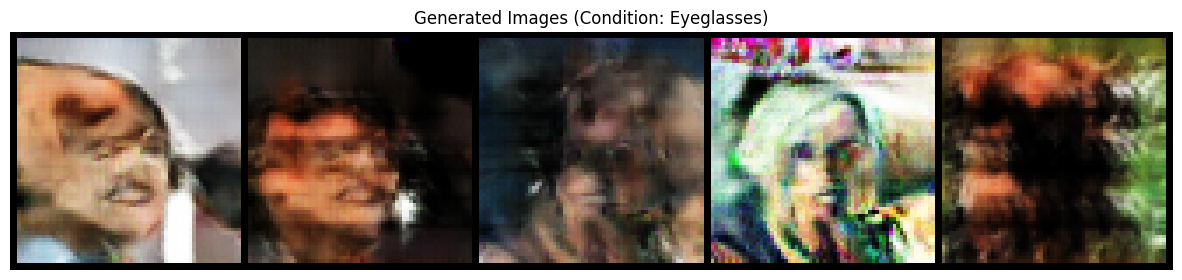
\includegraphics[width=1\textwidth]{test2_CGAN_30.png}
    \caption{Exemple avec attribut \texttt{Eyeglasses}}
    \label{fig:test2_CGAN_30}
\end{figure}

Sur la classe \texttt{Eyeglasses} qui est peu représentée dans le dataset, on obtient ici des images "glitchés" à cause du sur-apprentissage que l'on ne peut pas utiliser.

On remarque par ailleurs sur \ref{fig:test1_CGAN_30} que l'on a perdu en généralité, on reconnaît sur les 4 premières images la même personne et le 5ème avec la moustache apparaît aussi dans \ref{fig:test2_CGAN_30}.

\noindent\rule{\linewidth}{0.4pt}

\noindent On obtient un score LPIPS de $0.4689$ donc un a perdu en diversité par rapport

\noindent\rule{\linewidth}{0.4pt}

\subsubsection{Entraînement 15 époques (modèle final)}

On a vu qu'avec 30 époques, on a du sur-apprentissage, le modèle n'arrive plus à généraliser (diversité) et les images sont "glitchées" en raison de la répartition très inégale dans le dataset.

On va donc essayer de faire un entraînement sur 15 époques.

\medskip
\begin{lstlisting}[language=Python, caption={Entraînement du CGAN sur 15 époques}]
gen_15 = Generator(Z_DIM, C_DIM, FEATURES_GEN).to(device)
disc_15 = Discriminator(C_DIM, FEATURES_DISC).to(device)

NUM_EPOCHS = 15

G_losses_15, D_losses_15 = train_cgan(gen_15, disc_15, dataloader, device, num_epochs=NUM_EPOCHS, z_dim=Z_DIM)
\end{lstlisting}

\begin{figure}[H]
    \centering
    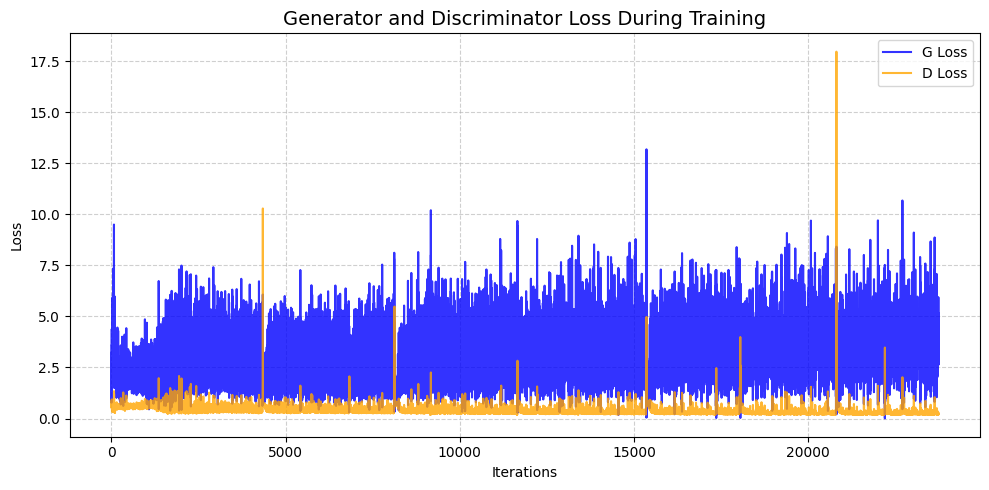
\includegraphics[width=1\textwidth]{loss_CGAN_15.png}
    \caption{Courbes de Loss du CGAN sur 15 époques}
    \label{fig:loss_CGAN_15}
\end{figure}

Contrairement à l'entraînement sur 30 époque, ici la loss ne diverge pas (\ref{fig:loss_CGAN_30}).

\begin{figure}[H]
    \centering
    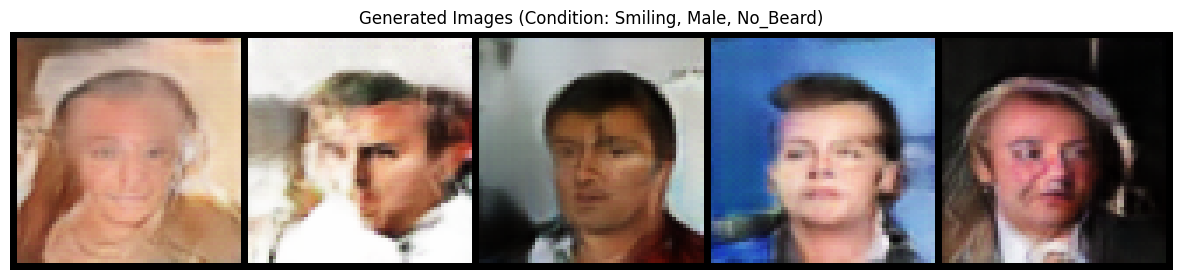
\includegraphics[width=1\textwidth]{test1_CGAN_15.png}
    \caption{Exemple avec attributs : \texttt{Smiling}, \texttt{Male} et \texttt{No\_Beard}}
    \label{fig:test1_CGAN_15}
\end{figure}

\begin{figure}[H]
    \centering
    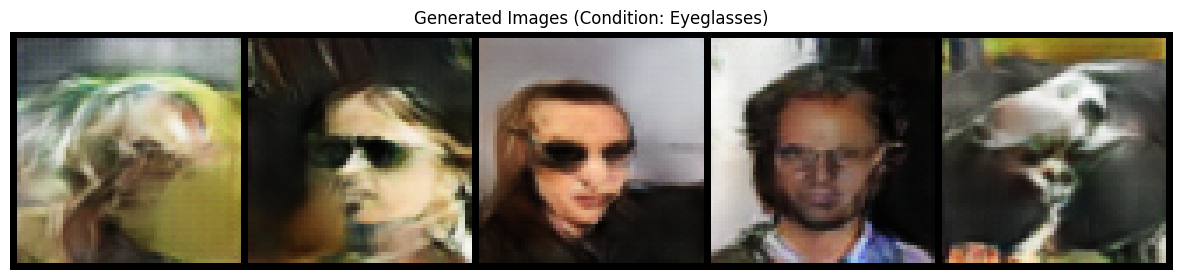
\includegraphics[width=1\textwidth]{test2_CGAN_15.png}
    \caption{Exemple avec attribut \texttt{Eyeglasses}}
    \label{fig:test2_CGAN_15}
\end{figure}

On remarque que l'on garde de la généralité et le modèle est plutôt efficace, même sur un attribut relativement peu représenté : \texttt{Eyeglasses} \ref{fig:test2_CGAN_15} (à seulement 20\%) on devine la présence de lunettes sur les images (images 2, 3 et 4) malgré quelques images "glitchées".

\noindent\rule{\linewidth}{0.4pt}

\noindent On obtient un score LPIPS de $0.5865$ donc similaire à l'entraînement sur 5 époques.

\noindent\rule{\linewidth}{0.4pt}

Les entraînements sont très longs (plusieurs heures), on ne va donc pas tester toutes les combinaisons d'hyperparamètres possibles. Etant donné que l'on a obtenu de bons résultats ici avec 15 époques, on va finalement garder ce modèle pour notre application cf. \ref{sec:streamlit}.


\subsubsection{Pistes d'améliorations}

Il pourrait être intéressant de faire de l'optimisation d'hyperparamètres avec un framework tel Optuna sur le modèle pour tenter de l'améliorer mais cela prendrait des jours et on se heurte à un problème quand il s'agit des modèles génératifs : quelle métrique à minimiser/optimiser choisir ?

\noindent En effet, puisque la Loss du Générateur et du Discriminateur jouent au chat et à la souris, une Loss basse pour l'un signifie une Loss haute pour l'autre, dans un environnement de recherche idéal, Optuna générerait des milliers d'images à la fin de chaque essai, calculerait le score FID (Fréchet Inception Distance), et chercherait à le minimiser. Cependant, cela prendrait des jours de calcul.

\noindent C'est pour cela que l'on utilise déjà les valeurs ``optim.Adam(gen.parameters(), lr=0.0002, betas=(0.5, 0.999))`` qui sont celles qui ont données les meilleurs résultats dans les papiers de recherche sur le CGAN.

\medskip

De plus, en remplaçant le bruit d'entrée du générateur une fois entraîné par un visage déterminé, on pourrait essayer de faire générer au modèle des images avec les attributs que l'on souhaite, par exemple prendre son propre visage et y ajouter des lunettes.

\newpage
\section{Le modèle CVAE}

\newpage
\section{Interface pour notre application (Inférence)}
\label{sec:streamlit}

Pour pouvoir faire facilement de l'inférence et tester notre projet, nous avons fait une interface streamlit dans \code{streamlit run app/app.py}.

Dans l'onglet GAN, on peut choisir les attributs que l'on veut voir apparaître sur les visages générés.

\begin{figure}[H]
    \centering
    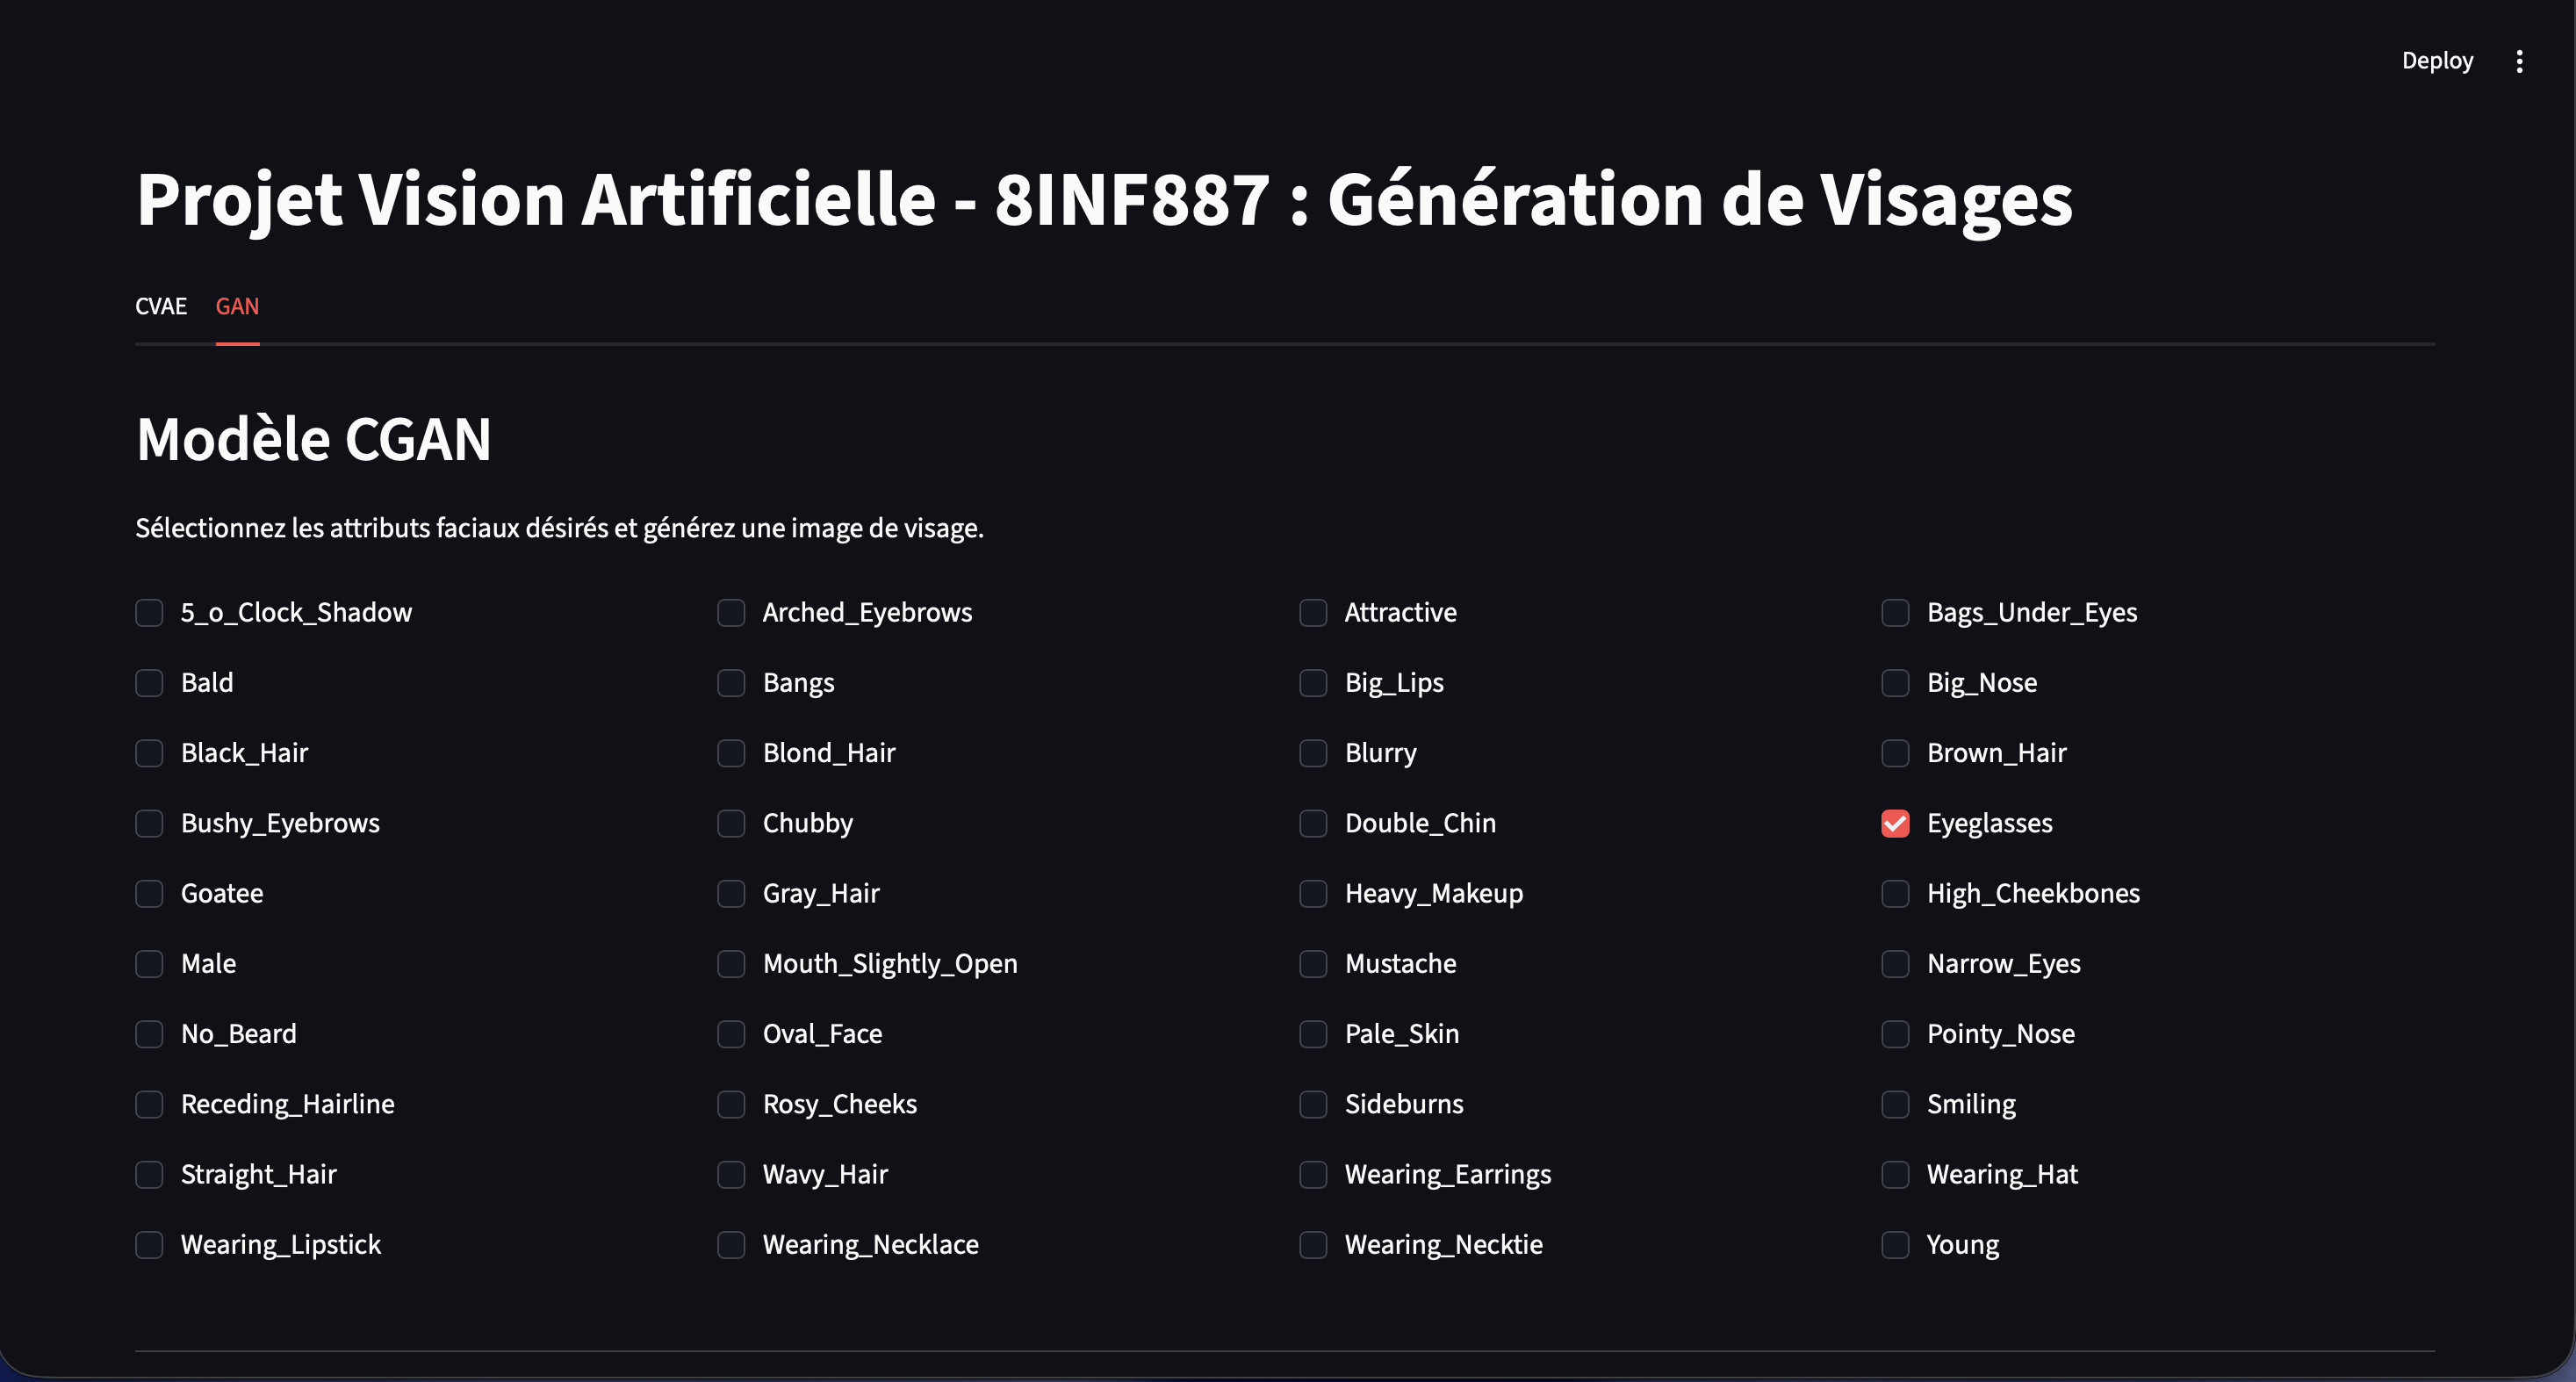
\includegraphics[width=1\textwidth]{streamlit_GAN_1.png}
    \caption{Interface streamlit GAN permettant de cocher les attributs, exemple avec Eyeglasses}
    \label{fig:streamlit_GAN_1}
\end{figure}

Ensuite, on peut choisir le nombre de visages à générer et les générer, le modèle utilise le fichier \code{GAN/saved\_models/cgan\_generator\_15.pth} qui contient les poids du modèle entraîné précédemment.

\begin{figure}[H]
    \centering
    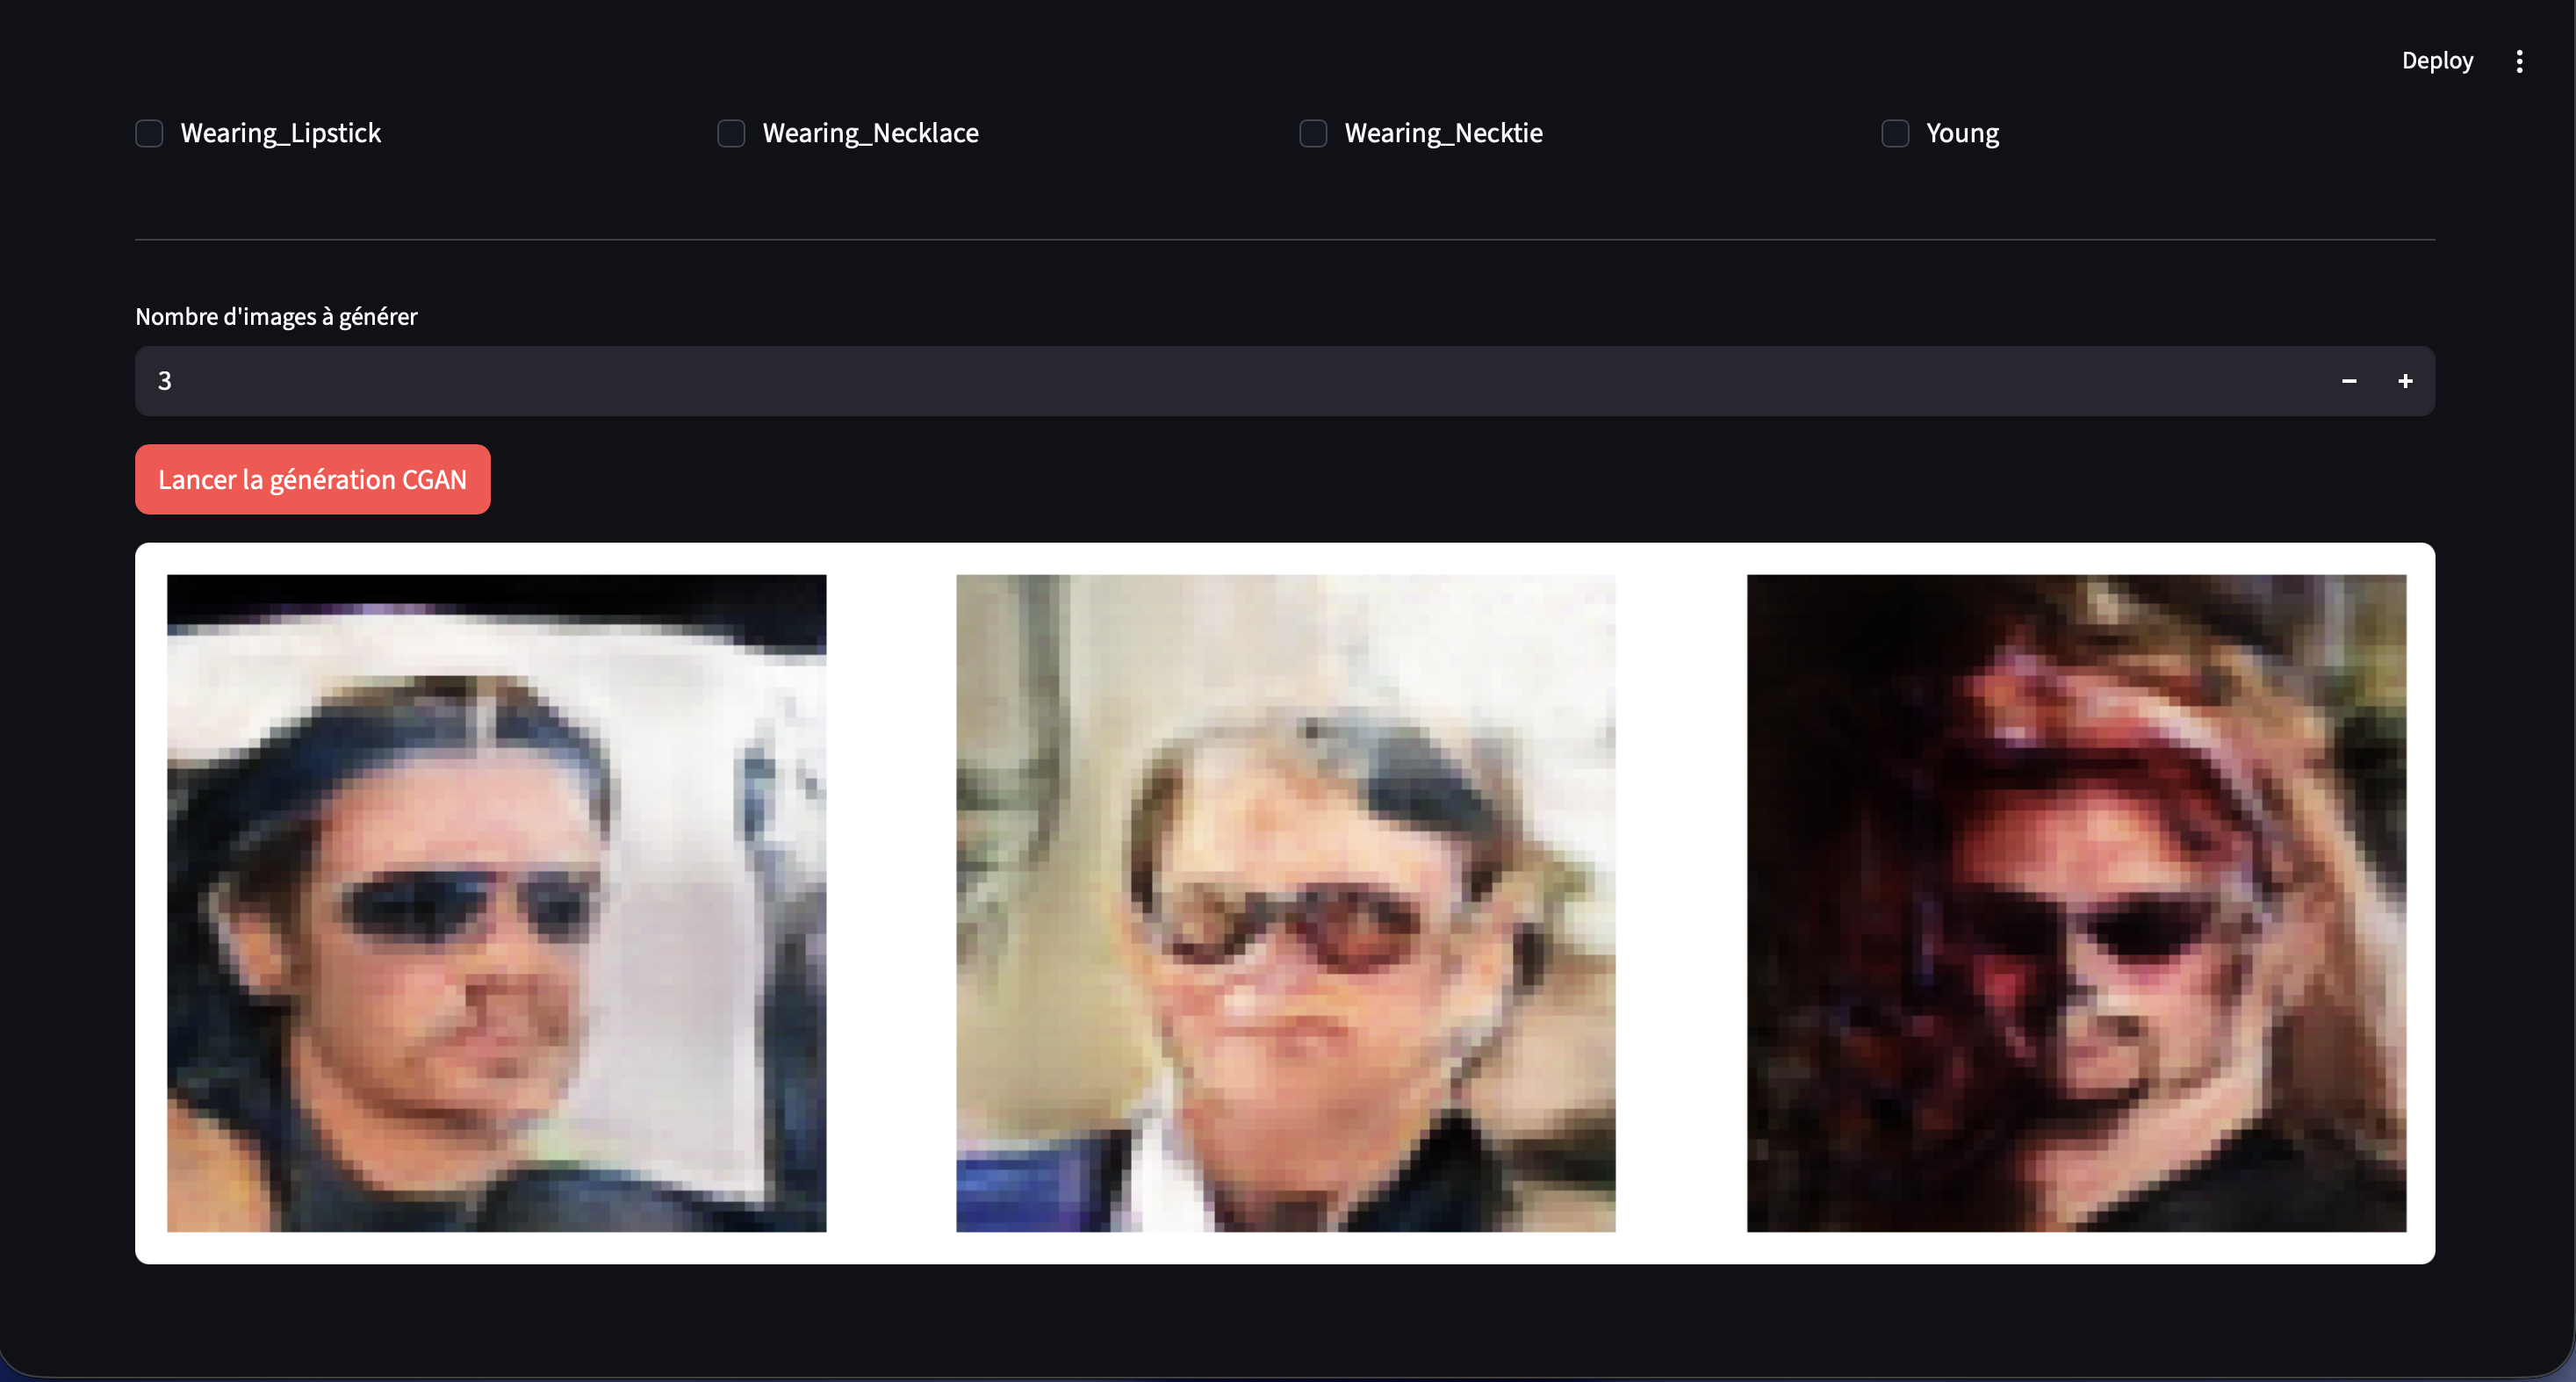
\includegraphics[width=1\textwidth]{streamlit_GAN_2.png}
    \caption{Interface streamlit GAN, génération de 3 visages}
    \label{fig:streamlit_GAN_2}
\end{figure}

Cela donne un exemple d'interface facilement utilisable pour notre projet.

\section{Conclusion}

% --------------------
\newpage
\section{Bibliographie}
\bibliographystyle{unsrt}
\bibliography{biblio}
% --------------------

\end{document}
